\documentclass[11pt,a4paper]{report}
\usepackage{amsmath}
\usepackage{amssymb}

\usepackage{graphicx}

\usepackage{listings}
\usepackage{color} %red, green, blue, yellow, cyan, magenta, black, white
\definecolor{mygreen}{RGB}{28,172,0} % color values Red, Green, Blue
\definecolor{mylilas}{RGB}{170,55,241}


\usepackage{graphicx}


\begin{document}
\begin{center}

\LARGE Mek4250 - Mandatory assignment 2
\\
Andreas Thune
\\
\LARGE
8.05.2016

\end{center}
\textbf{Exercise 1}
\\
7.1) Given the following weak formulation of Stokes problem:
\begin{align*}
a(u,v)+b(p,v)&=(f,v) \ \forall \ v \in H_0^1(\Omega)^d\\
b(q,u)&=0 \ \forall q \in L^2(\Omega)
\end{align*}
Where $a(u,v) = \int_{\Omega}\nabla u : \nabla v dx$ and $b(p,v) =\int_{\Omega} p\nabla \cdot v dx$.
\\
We then want to show the following conditions required for well-posedness:
\begin{align}
&a(u,v) \leq C_1 ||u||_{H^1(\Omega)}||v||_{H^1(\Omega)} \ \forall \ v,u \in H_0^1(\Omega)\\
&a(u,u) \geq D||u||_{H^1(\Omega)}^2 \ \forall \ u \in H_0^1(\Omega)\\
&b(q,u) \leq C_2||u||_{H^1(\Omega)}||q||_{L^2(\Omega)} \ \forall \ u \in H_0^1(\Omega), \ \forall q \in L^2(\Omega)
\end{align}
Note that $u$ and $v$ are vector functions. To show the three conditions I will use the notation $u(x)=[u^1(x),...,u^d(x)]$, for $x \in  \mathbb{R}^d$. We must also remember that the inner product $":"$ in the $a$ form is defined as 
\begin{align*}
\nabla u : \nabla v = \Sigma_{i=1}^d\Sigma_{j=1}^d u_{x_j}^i(x)v_{x_j}^i(x)
\end{align*}
It is also be helpful to define the $H^1$ norm for vector functions:
\begin{align*}
||u||_{H^1(\Omega)}^2 &= ||u||_{L^2(\Omega)}^2 + |u|_{H^1(\Omega)}^2 \\
||u||_{L^2(\Omega)}^2 &= \sum_{i=1}^d ||u^i||_{L^2(\Omega)}^2 \\
|u|_{H^1(\Omega)}^2 &= \sum_{i=1}^d |u^i|_{H^1(\Omega)}^2= \sum_{i=1}^d\sum_{j=1}^d ||u_{x_j}^i||_{L^2(\Omega)}^2
\end{align*}
These definitions give us the inequalities $ |u^i|_{H^1} \leq |u|_{H^1}$ and \\$||u_{x_j}^i||_{L^2}\leq |u^i|_{H^1} $.
\\
\textbf{Inequality (1)}
\begin{align*}
a(u,v)&= \int_{\Omega}\nabla u : \nabla v dx=\int_{\Omega}\sum_{i=1}^d\sum_{j=1}^d u_{x_j}^iv_{x_j}^idx \\
&=\sum_{i=1}^d\sum_{j=1}^d (u_{x_j}^i,v_{x_j}^i)_{L^2(\Omega)} \\
&\leq \sum_{i=1}^d\sum_{j=1}^d ||u_{x_j}^i||_{L^2(\Omega)}||v_{x_j}^i||_{L^2(\Omega)} \ \text{  using Cauchy-Schwartz inequality}  \\
&\leq d \sum_{i=1}^d |u^i|_{H^1(\Omega)}|v^i|_{H^1(\Omega)} \ \text{ since $||u_{x_j}^i||_{L^2} \leq |u^i|_{H^1}$} \\
&\leq d^2 |u|_{H^1(\Omega)}|v|_{H^1(\Omega)} \ \text{        using $|u^i|_{H^1} \leq |u|_{H^1}$} \\
&\leq d^2 ||u||_{H^1(\Omega)}||v||_{H^1(\Omega)} \ \text{    since $|u|_{H^1}\leq ||u||_{H^1}$ } 
\end{align*}
\\
\textbf{Inequality (2)}
\\
Using the Poincares inequality for $H_0^1(\Omega)$, given by: 
\begin{align*}
|u|_{H^1(\Omega)}^2\geq C||u||_{L^2(\Omega)}^2
\end{align*} 
we get 
\begin{align*}
a(u,u)&= \int_{\Omega}\nabla u : \nabla u dx=\int_{\Omega}\sum_{i=1}^d\sum_{j=1}^d u_{x_j}^iu_{x_j}^idx \\
&=\sum_{i=1}^d\sum_{j=1}^d ||u_{x_j}^i||_{L^2(\Omega)}^2=\sum_{i=1}^d |u^i|_{H^1(\Omega)}^2\\
&= \sum_{i=1}^d\frac{1}{2}(|u^i|_{H^1(\Omega)}^2+|u^i|_{H^1(\Omega)}^2) \\
&\geq \sum_{i=1}^d\frac{1}{2}(|u^i|_{H^1(\Omega)}^2+C||u^i||_{L^2(\Omega)}^2) \\
&\geq \frac{min\{1,C\}}{2}\sum_{i=1}^d(|u^i|_{H^1(\Omega)}^2+||u^i||_{L^2(\Omega)}^2) \\
&= \frac{min\{1,C\}}{2}||u||_{H^1(\Omega)}^2=D||u||_{H^1(\Omega)}^2
\end{align*}
\\
\textbf{Inequality (3)}
\begin{align*}
b(q,u)&=\int_{\Omega} q\nabla \cdot u dx=\int_{\Omega}\sum_{i=1}^d qu_{x_i}^i dx \\
&\leq \sum_{i=1}^d ||q||_{L^2(\Omega)} ||u_{x_i}^i||_{L^2(\Omega)} \ \text{  using Cauchy-Schwartz inequality}  \\
&\leq ||q||_{L^2(\Omega)}\sum_{i=1}^d |u^i|_{H^1(\Omega)} \\
&\leq d||q||_{L^2(\Omega)}|u|_{H^1(\Omega)} \\
&\leq d||q||_{L^2(\Omega)}||u||_{H^1(\Omega)}
\end{align*}
\\
7.6) Want to solve the the stokes problem with a manufactured solution $ue(x,y)=(\sin(\pi y),\cos(\pi x))$ and $pe(x,y)=\sin(2\pi x)$ on $\Omega = (0,1)^2$. This means solving the problem:
\begin{align*}
-\Delta u - \nabla p &= f \\
\nabla \cdot u &= 0 \\
u &= ue \ \text{on } \partial\Omega_D \\
-\frac{\partial u}{\partial n} - pn &= h \ \text{on } \partial\Omega_N
\end{align*} 
To be able to solve the equation we need to define $\partial\Omega_D$ and $\partial\Omega_N$, as well as deriving $f$ and $h$. 7.7 use $\partial\Omega_N= \{y=0\}$ and $\partial\Omega_D=\partial\Omega - \partial\Omega_N$. This gives us $h=(-\pi,-sin(2\pi x))$. We see this by noting that $n=(0,-1)$ on $\partial\Omega_N$, and calculating:
\begin{align*}
h &= -\frac{\partial u(x,0)}{\partial n} - p(x,0)n  = -(\nabla u_1\cdot n,\nabla u_2\cdot n) -\sin(2\pi x)n\\
&= -( [0,\pi \cos(\pi \cdot0)] \cdot[0,-1], ( [-\pi \sin(\pi x),0]\cdot[0,-1]) +(0,-\sin(2\pi x)) \\
& = (-\pi,0)+(0,-\sin(2\pi x)) = (-\pi,-\sin(2\pi x))
\end{align*}
Now lets find $f$:
\begin{align*}
f &= -\Delta u - \nabla p \\
&= (\pi^2 \sin(\pi y),\pi^2 \cos(\pi x)) - (2\pi\cos(2\pi x),0) 
\end{align*} 
The last step before implementing the numerics is to derive the variational form:
\begin{align*}
-\int_{\Omega} \Delta u \cdot v  dx - \int_{\Omega} \nabla p \cdot v  dx &= \int_{\Omega} \nabla u :\nabla v  dx + \int_{\Omega} p \nabla\cdot v  dx -\int_{\partial\Omega_n}(\frac{\partial u}{\partial N} + pn)\cdot v  dS \\
&=\int_{\Omega} \nabla u :\nabla v  dx + \int_{\Omega} p \nabla\cdot v  dx +\int_{\partial\Omega_N}h\cdot v  dS 
\end{align*}
Together with the deivergence term this gives us the following variational form:
\begin{align*}
\int_{\Omega} \nabla u :\nabla v \ dx + \int_{\Omega} p \nabla\cdot v \ dx +\int_{\Omega} q\nabla\cdot u  \ dx = \int_{\Omega} f\cdot v \ dx +\int_{\partial\Omega_N}h\cdot v \ dS 
\end{align*}
As usual this should hold $\forall$ $v \in \{ v \in H^1(\Omega)^2 : v|_{\partial\Omega_D} =0  \}$ and $\forall$ $q \in L^2(\Omega)$. We also deal with the Dirichlet boundary condition in the normal way (ignoring them, and fixing the system). 
\\
\\
The FEniCS implementation of this problem using the four combinations of elements asked for in the exercise is added at the end of the assignment. We were then asked to test if our approximations converged at the expected rate. The natural way of measuring the error is using $H^1$ norm for velocity and $L^2$ norm for pressure. The theoretical convergence rate is then given by the following inequality:
\begin{align*}
||u-u_h||_{H^1}+||p-p_h||_{L^2} \leq Ch^{q}||u||_{H^{q+1}}+Dh^{t+1}||p||_{H^{t+1}}
\end{align*}
Here $q$ and $t$ are the degrees of the elements used in our finite element spaces. Using $h=\{\frac{1}{8},\frac{1}{16}, \frac{1}{32},\frac{1}{64}\}$ I got the following results using least squares:
\begin{center}
    \begin{tabular}{| l | l | l |}
    \hline
     & Convergence rate & Constant  \\ \hline
    $P4-P3$ & 4.045257 & 0.084663 \\ \hline
    $P4-P2$ & 2.902867 &  0.493978	\\ \hline
    $P3-P2$ & 2.890269 & 0.447429\\ \hline
    $P3-P1$ & 2.024947 &  1.135217	\\ \hline
    \end{tabular}
\end{center}
I justify using least squares by doing a loglog plot of the error and the mesh resolution for the different element types. We see that the loglog plot is straight lines for all elements, and using least squares therefore makes sense.
\begin{figure}
  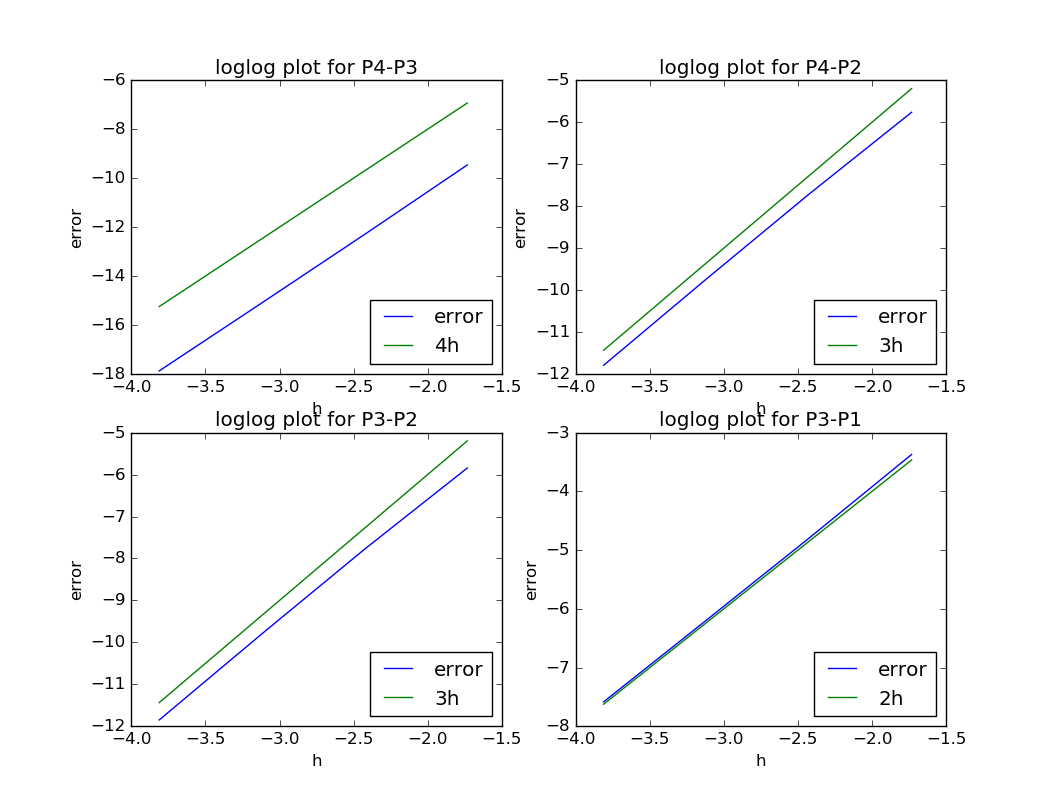
\includegraphics[width=\linewidth]{element_con.png}
  \caption{loglog plot for the error plotted together with linear functions with the expected steepness. Observe that the slope of the expected line and the error plot are almost the same for all element combos}
  \label{Fig 1}
\end{figure}
\\
\\
7.7) The wall shear stress is defined in the exercise. Set \\$\Gamma = \{(x,y) \in \Omega | x=0 \}$, and the unit vector $t=[0,1]$ parallel to $\Gamma$, the wall shear stress is then given as: 
\begin{align*}
||\nabla u\cdot t||_{L^2(\Gamma)}^2 &= \int_{\Gamma} |\nabla u \cdot t|^2  \ dS \\
&=  \int_{\Gamma} |(\nabla u_1 \cdot t,\nabla u_2 \cdot t)|^2  \ dS \\
&=\int_{\Gamma} \frac{\partial u_1}{\partial y}^2 + \frac{\partial u_2}{\partial y}^2 \ dS
\end{align*} 
Using this I calculated the convergence rate for different element combos, by solving the equation for the same mesh resolutions as in 7.6. To calculate the convergence rates I used least squares, and the results were as follows:
\begin{center}
    \begin{tabular}{| l | l | l |}
    \hline
     & Convergence rate & Constant   \\ \hline
    $P4-P3$ & 3.999511 & 0.011619    \\ \hline
    $P4-P2$ & 3.999512 & 0.011619	\\ \hline
    $P3-P2$ & 2.999236 & 0.077591    \\ \hline
    $P3-P1$ & 2.999236 & 0.077591	\\ \hline
    	$P4-P1$ & 3.999512 & 0.011619	\\ \hline
    \end{tabular}
\end{center}
These results seems to indicate the following convergence result for wall shear stress:
\begin{align*}
||\nabla (u-u_h)\cdot t||_{L^2(\Gamma)} \leq Ch^q
\end{align*} 
Where $q$ is equal to the degree of the element used for velocity, and both the constant $C$ and $q$ is independent of the pressure element. I solved the equation using $P4-P1$ elements to show that this relation also holds for element combos where the diffrence in degree is bigger then $2$. As in exercise 7.6 I have added a loglog plot to justify use of least squares.
\begin{figure}
  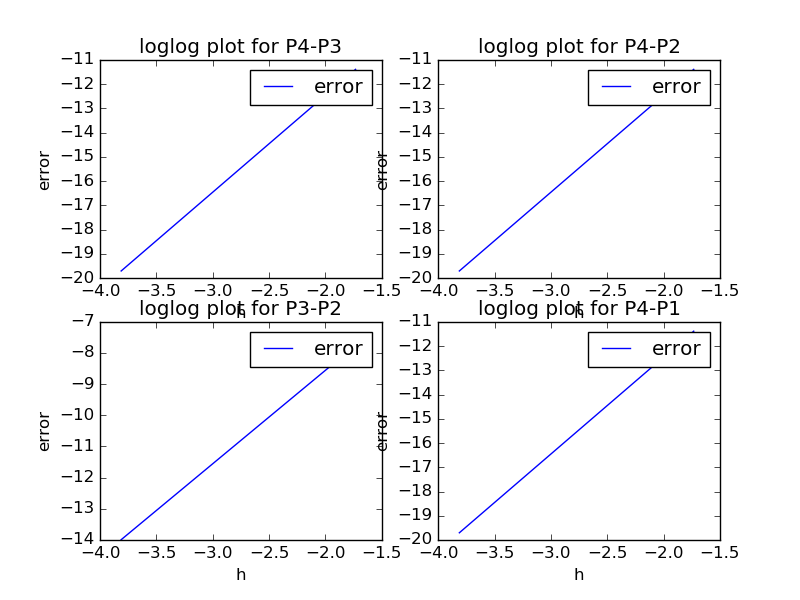
\includegraphics[width=\linewidth]{stress_con.png}
  \caption{loglog plot for the wall shear stress error $||\nabla (u-u_h)\cdot t||_{L^2(\Gamma)}$. Observe that lines are almost linear.}
  \label{Fig 2}
\end{figure}
\\
\\
\textbf{Exercise 2}
\\
a) We are given a function $\Phi(x,y)=\sin(\pi xy)$ and asked to find the source term $f$ such that solving our equation yields the solution:
\begin{align*}
ue(x,y)=[\frac{\partial \Phi}{\partial y},-\frac{\partial \Phi}{\partial y}]= \pi[x\cos(\pi xy),-y\cos(\pi xy)]
\end{align*}
Our equation is 
\begin{align*}
-\mu \Delta u -\lambda\nabla\nabla\cdot u &= f \ \text{in } \Omega=(0,1)^2 \\
u&=ue \ \text{in } \partial\Omega
\end{align*}
Since $\nabla\cdot ue=0$, the source term $f$ is given by $f=-\mu \Delta ue$. To make it simple I choose to derive $f$ using sympy. The code is added at the end. Setting $v=[\cos(\pi xy),\sin(\pi xy)]$, I found the following expression for $f$:
\begin{align*}
f &= -\mu\pi[\Delta x\cos(\pi xy),-\Delta y\cos(\pi xy)] \\
&= -\mu\pi^2[-v\cdot [\pi x^3+\pi xy^2,2y],v\cdot [\pi y^3+\pi x^2y,2x]]
\end{align*}
b) I have computed the errors between exact and numerical solution in the code at the end. The results are given as output in the code. For simplicity I set $\mu=1$.
\\
\\
The variational form of this equation is
\begin{align*}
\mu\int_{\Omega} \nabla u\nabla v dx + \lambda\int_{\Omega} \nabla u\cdot\nabla\cdot v dx = \int_{\Omega} f\cdot v dx
\end{align*}
An alternative way of solving this equation is to set $p=\lambda\nabla\cdot u$, and then it as a mixed problem. When we do this we avoid the problems that I discuss below, however since the exercise does not explicitly ask for it, I will not implement this version.
\\
\\
c) We were then asked to calculate the convergence rate of the finite element method for this equation using the mesh resolutions given in the exercise. I did this using least squares, and below follows a table of the $L^2$ and $H^1$ convergence rates I got when using $P1$ elements:
\begin{center}
    \begin{tabular}{| l | l | l | l | l |}
    \hline
     & $L^2$ con. rate& Constant $L^2$ & $H^1$ con. rate& Constant $H^1$\\ \hline
     $\lambda=1$& 1.975326 & 2.213178 & 0.997337& 7.621186 \\ \hline
     $\lambda=100$& 1.369169 & 3.795261& 1.208202& 23.611052\\ \hline
     $\lambda=10000$& 0.108859 & 0.567093 & 0.146335 & 5.043682 \\ \hline
    \end{tabular}
\end{center}
The same for $P2$ elements:
\begin{center}
    \begin{tabular}{| l | l | l | l | l |}
    \hline
    & $L^2$ con. rate& Constant $L^2$ & $H^1$ con. rate& Constant $H^1$\\ \hline
     $\lambda=1$& 3.019367 & 0.386373 & 1.994832& 3.920336 \\ \hline
     $\lambda=100$& 3.570446 & 7.716594 & 2.452345& 33.981253 \\ \hline
     $\lambda=10000$& 2.252270 & 1.596042 & 1.260810& 9.058619 \\ \hline
    \end{tabular}
\end{center}
Locking is defined as loosing converging rate when $\lambda>>\mu$. For $P1$ elements we see that the $L^2$ convergence drops by almost 1 for $\lambda=100$, and by almost 2 for  $\lambda=10000$. The $H^1$ convergence on the other hand only drops for $\lambda=10000$, while it for $\lambda=100$ actually is higher than we would expect. For $\lambda=1$, everything behaves nicely.
\\
\\
For $P2$ elements we observe locking for both $L^2$ and $H^1$, i.e. a convergence drop of almost 1, but only when $\lambda=10000$. For $\lambda=100$ the convergence rate is higher than what we would expect. One could note, that where we see increased convergence we also see big constants. Again for $\lambda=1$ everything looks normal. 
\begin{figure}
  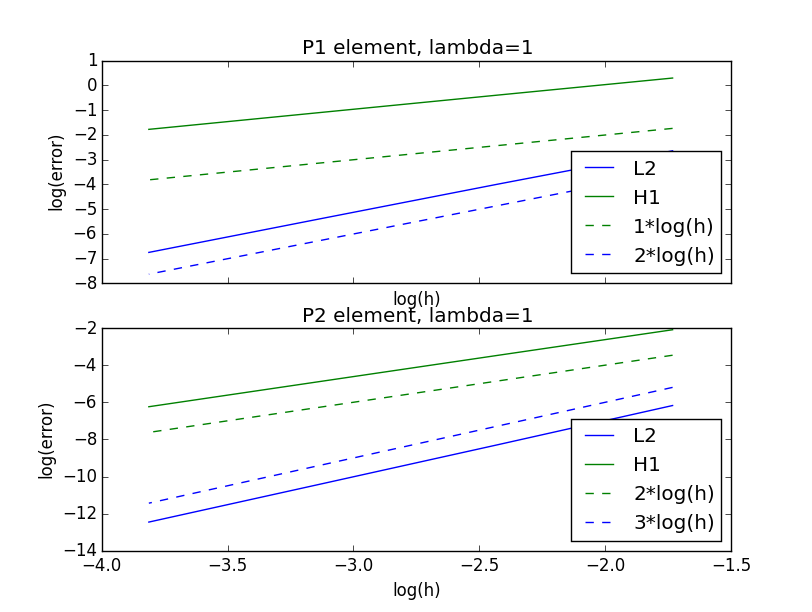
\includegraphics[width=\linewidth]{l1.png}
  \caption{For $\lambda =1$, we see that both the $L^2$ and $H^1$ error behave as expected, i.e. the error lines are almost parallel with the lines representing theoretical convergence rate.}
  \label{Fig 3}
\end{figure}


\begin{figure}
  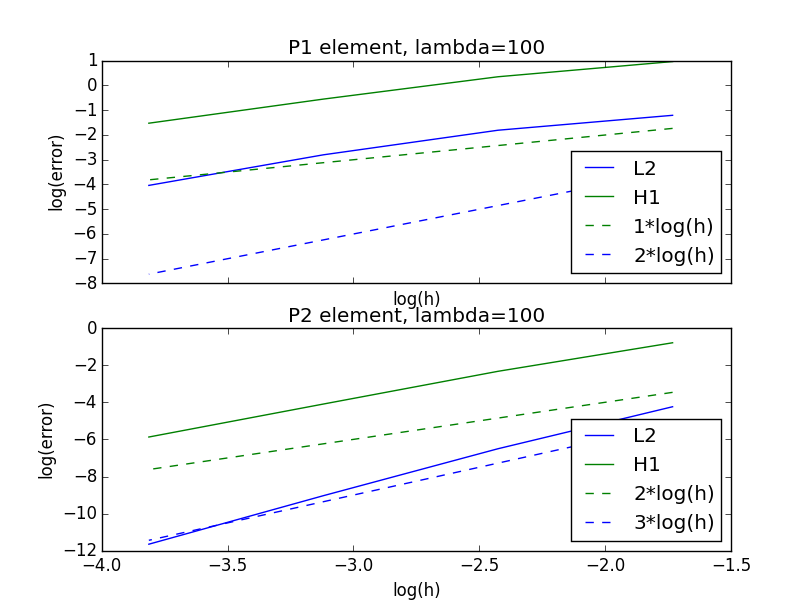
\includegraphics[width=\linewidth]{l100.png}
  \caption{For $\lambda =100$, we observe that the $L^2$ error for $P1$ elements line have almost 1 less in slope than what is expected. For the other lines, the behavior is as expected or better. }
  \label{Fig 4}
\end{figure}


\begin{figure}
  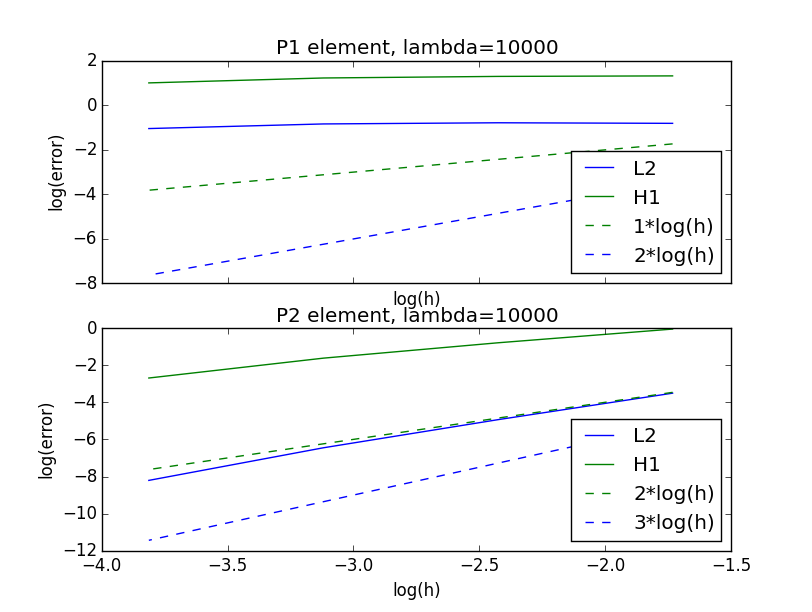
\includegraphics[width=\linewidth]{l10000.png}
  \caption{For $\lambda =10000$, wee see that all error lines have smaller slope then expected, but the the situation is a lot worse for $P1$ elements.}
  \label{Fig 5}
\end{figure}
\end{document}